
\chapter{Exp\'erimentations~: Comparaisons de \ppff\ avec Java et FastFlow}
\label{experiences.chap}

Ce chapitre pr\'esente une \'evaluation exp\'erimentale de la biblioth\`eque \TT{PpFf} afin de comparer ses performances avec d'autres approches d'ex\'ecution parall\`ele, plus sp\'ecifiquement avec \TT{Java} et \TT{FastFlow}.
%
Dans les sections~\ref{wordcount.sect} et~\ref{stockprice.sect}, nous pr\'esentons deux applications \'ecrites avec \PpFf. Ces applications ont \'et\'e choisies non seulement pour montrer certaines fonctionnalit\'es de notre biblioth\`eque, mais \'egalement pour leur pertinence dans des sc\'enarios typiques. La section~\ref{wordcount.sect} pr\'esente une application permettant de calculer le nombre d'occurrences des mots dans un texte --- le <<\emph{Hello World!}>> des syst\`emes de traitement de donn\'ees en mode \emph{batch} --- alors que la section~\ref{stockprice.sect} pr\'esente une application permettant de calculer des statistiques sur les prix d'indices boursiers --- un exemple typique de traitement de flux en ligne (\emph{online data processing}). Mais tout d'abord, nous pr\'esentons la fa\c{c}on dont nos exp\'erimentations ont \'et\'e effectu\'ees.

%Finalement, la section~\ref{coutsPpFf.sect} pr\'esente une application permettant de d\'eterminer les surco\^uts introduits par \TT{PpFf} par rapport \`a \TT{FastFlow} --- un \emph{micro benchmark} consistant en un pipeline avec un seul op\'erateur. 



\section{M\'ethode utilis\'ee pour les exp\'erimentations}
\label{usedMethodsForBenchmarks.chap}

\subsection{Caractéristiques des machines et compilateurs utilisés}

Chaque syst\`eme informatique a des caract\'eristiques propres. Quelques-uns des facteurs qui influencent les performances d'un tel syst\`eme sont le type de processeur, le nombre de processeurs ou de c\oe{}urs, et la vitesse des processeurs. 


\newcommand{\LARGEUR}{3cm}

\begin{table}
\begin{tabular}{|p{3cm}|p{\LARGEUR}|p{\LARGEUR}|p{\LARGEUR}|}
\hline
  & \M1 & \M2 & \M3
\\\hline
\textbf{OS} & CentOS 7.8.2003 & CentOS 7.8.2003 & CentOS 7.6.1810
\\\hline
\textbf{Architecture} &  x86\_64 & x86\_64 & x86\_64
\\\hline
\textbf{Type de processeur} & GenuineIntel  & AuthenticAMD & GenuineIntel
\\\hline
\textbf{Vitesse du processeur (GHz)} & 2.66 & 2.30 & 3.96
\\\hline
\textbf{Mono/multi-usager} & Multi & Multi & Mono
\\\hline
\textbf{Nb.~coeurs physiques} & 16 & 32 & 4
\\\hline
\textbf{Nb.~coeurs logiques} & 16 & 64 & 8
\\\hline
\texttt{java}
  & \texttt{openjdk 11.0.7 2020-04-14 LTS}
  & \texttt{java version "1.8.0\_51"}
  & \texttt{openjdk version "11.0.7" 2020-04-14 LTS}
\\\hline
\texttt{g++ (GCC)}
   & 8.3.1
   & 8.3.1 
   & 8.3.0
\\\hline
\end{tabular}
\caption[Les caract\'eristiques des machines utilis\'ees dans nos exp\'eriences.]{Les caract\'eristiques des machines utilis\'ees dans nos exp\'eriences. Le tableau d\'ecrit pour chaque machine le syst\`eme d'exploitation utilis\'e, le type de la machine (mono- ou multi-usager), le nombre de coeurs (physiques vs.\ logiques) et les versions des compilateurs utilis\'es dans nos exp\'eriences.}
\label{machines.table}
\end{table}


Afin d'avoir des r\'esultats plus représentatifs, nous avons conduit nos exp\'eriences sur trois machines diff\'erentes. Le tableau~\ref{machines.table} montre les caract\'eristiques de ces machines. Les machines \M1 et \M2 sont des machines multi-usagers, tandis que la machine \M3 est une machine mono-usager sur laquelle les exp\'eriences ont \'et\/e roul\'ees sans interf\'erence.

\subsection{Choix des programmes comparés}

Le fonctionnement des programmes \TT{Java}, \TT{PpFf} et~\TT{FastFlow} n'est pas le m\^eme. Alors que \TT{PpFf} et \TT{FastFlow} permettent de varier le nombre de fils d'ex\'ecution (\emph{threads}), \TT{Java} ne le permet pas. Afin de montrer les meilleurs temps d'ex\'ecution et l'\'evolutivit\'e de \TT{PpFf}, des exp\'eriences pr\'eliminaires ont \'et\'e effectu\'ees, sur chaque machine, pour identifier les meilleures versions, et ce tant pour \TT{PpFf} que pour \TT{Java} et \TT{FastFlow}.
Ces exp\'eriences pr\'eliminaires ont \'et\'e conduites avec un nombre de r\'ep\'etitions de 10 et avec une quantit\'e <<moyenne>> de donn\'ees. 

Dans le cas de \TT{PpFf} et \TT{FastFlow}, l'objectif \'etait de d\'eterminer le meilleur niveau de parall\'elisme \`a utiliser dans les \emph{farm}s, c'est-\`a-dire, pour \TT{PpFf}, la valeur pour la m\'ethode \TT{parallel()}, pour le parall\'elisme de donn\'ees.
%
Par contre, dans le cas de \TT{Java}, l'objectif était de comparer trois versions~: sans \emph{warmup} et avec ou sans \emph{JIT}, avec \emph{warmup} et \emph{JIT} (voir ci-bas).
%
C'est la version avec \emph{warmup} et \emph{JIT} qui a \'et\'e utilis\'ee.


L'effet de pr\'echauffage (\emph{warmup} en anglais) est g\'en\'eralement d\^u au chargement des classes et \`a l'interpr\'etation du \emph{bytecode} au d\'emarrage du programme plutôt qu'à l'exécution directe d'instructions machines. Lorsqu'une nouvelle application d\'emarre, toutes les classes requises sont charg\'ees en m\'emoire par le mod\`ele de chargement paresseux (\emph{lazy loading} en anglais). Un tel mod\`ele est couramment utilis\'e pour reporter l'initialisation d'un objet jusqu'au moment o\`u il est n\'ecessaire.
%
\label{jitDescription.sect}
%
Il y a aussi l'effet de la compilation 
\emph{JIT}~\citep{cramer1997compiling} (\emph{Just-In-Time compiler}),
%
un composant de l'environnement d'ex\'ecution Java qui am\'eliore les performances des applications en compilant le \emph{bytecode} de la machine virtuelle en code machine \emph{au moment de l'ex\'ecution}. Le \emph{bytecode} est l'ensemble des instructions de la \emph{JVM} (\emph{Java Virtual Machine}) qui permet aux applications d'\^etre ex\'ecut\'ees sur plusieurs plates-formes. La conversion du \emph{bytecode} en langage machine a un impact positif significatif sur la vitesse d'ex\'ecution une fois que le code machine s'exécute directement.

Dans toutes nos exp\'eriences, les programmes \TT{Java} comparés avec \ppff\ ont donc \'et\'e pr\'echauff\'es en lan\c{c}ant une proc\'edure de pr\'echauffage avant de mesurer le temps pour la portion de code pertinente. Cette proc\'edure de pr\'echauffage a consisté à faire un traitement préalable des données avec presque toutes les m\'ethodes utilis\'ees.

\subsection{Temps mesurés}
 
Il faut noter que le temps mesur\'e dans toutes les exp\'eriences \emph{exclut le lancement du programme}. La mesure du temps se fait de l'int\'erieur du programme m\^eme, une fois celui-ci lanc\'e. Lorsque le traitement est termin\'e, le temps est \'emis en sortie du programme sur \TT{stdout}. Donc, le temps n'est pas mesur\'e avec la commande <<\TT{time}>>. Notamment, dans le cas de \TT{Java}, cela exclut le temps de lancement de la machine virtuelle. De plus, les quantit\'es de donn\'ees utilis\'ees dans les exp\'eriences ont \'et\'e choisies de sorte que les temps d'ex\'ecution soient d'au moins 200 millisecondes.


\subsection{Exemples d'expériences préliminaires}

\graphe{WordCount-temps-java-2-10}{Temps PpFf}
\graphe{WordCount-log-temps-java-2-10}{Temps PpFf (log)}

Afin de montrer les \'etapes des diverses exp\'eriences qui ont conduit aux r\'esultats finaux, l'annexe~\ref{ExperiencesPreliminairesWordCount.ann} pr\'esente un extrait d'un fichier de configuration \TT{WordCount-bm-config.rb}, utilis\'e pour l'ex\'ecution des expériences, alors que les figures~\grapheref{WordCount-temps-java-2-10} et~\grapheref{WordCount-log-temps-java-2-10} présentent quelques-uns des r\'esultats préliminaires obtenus.

Cr\'e\'e par mon directeur de recherche, ce script permet de configurer les expériences \`a ex\'ecuter. Dans ce fichier on peut sp\'ecifier tous les param\`etres dont on a besoin : la machine pour laquelle est définie l'expérience, les quantités de donn\'ees, le nombre de r\'ep\'etitions, et les programmes \`a ex\'ecuter. Les donn\'ees sont regroup\'ees par taille en diverses cat\'egories, les plus importantes étant \TT{donnees\_preliminaires}, \TT{pas\_mal\_de\_donnees} et \TT{beaucoup\_de\_donnees}. Les deux premi\`eres cat\'egories ont servi pour d\'eterminer les meilleures versions \`a utiliser pour chacun des programmes. Par exemple, les graphes des figures~\grapheref{WordCount-temps-java-2-10} et~\grapheref{WordCount-log-temps-java-2-10} montrent les temps d'ex\'ecution pour \TT{WordCount} --- avec échelle linéaire vs.\ logarithmique --- sur la machine \M1 pour le programme \TT{PpFf} en utilisant la premi\`ere cat\'egorie de donn\'ees (expérience no.~2). Les temps sont en millisecondes (ms), obtenus en prenant la moyenne de 10 ex\'ecutions.  Trois  s\'eries de mesures ont \'et\'e effectu\'ees : \TT{PpFf-1} avec une seule instance parallèle d'un \emph{farm}, \TT{PpFf-2} avec deux et \TT{PpFf-3} avec trois.


L'objectif de ces mesures pr\'eliminaires est de d\'eterminer la valeur qui semble la meilleure pour les temps d'ex\'ecution. On peut observer que le temps d'ex\'ecution pour \TT{PpFf-3} est beaucoup plus grand que les deux autres (figure~\grapheref{WordCount-temps-java-2-10}).
%
Pour mieux distinguer les performances entre les deux autres versions de \TT{PpFf}, une échelle logarithmique peut aussi être utilis\'ee (figure~\grapheref{WordCount-log-temps-java-2-10})~: on peut constater que \TT{PpFf-2}, avec deux instances parall\`eles d'un \emph{farm}, est plus performant que \TT{PpFf-1}, avec une seule instance. 
%
\TT{PpFf-2} est donc la version qui sera compar\'ee aux autres programmes lors des expériences finales sur la machine \M1. Ces expériences comparent donc les meilleures versions entre elles, en utilisant de plus grandes quantit\'es de donn\'ees et avec un plus grand nombre de r\'ep\'etitions, soit 40.


Le nombre de r\'ep\'etitions indique combien de fois chaque programme est exécuté et son temps mesuré.
%
On calcule ensuite la moyenne et l'écart-type. Dans un graphe comme celui de la figure~\grapheref{WordCount-temps-java-2-10}, les moyennes sont repr\'esent\'ees par les valeurs qui composent la courbe sur le graphe et les dispersions par des petits barres verticales (par ex., voir les valeurs pour \TT{PpFf-3}
de la figure~\grapheref{WordCount-temps-java-2-10}). Plus précisément, la barre verticale indique un intervalle de 2 écart-types, donc un intervalle qui contient approximativement 95~\% des mesures.

Chaque s\'erie des exp\'eriences finales inclut le programme \TT{Seq}, une version s\'equentielle utilisant les m\^emes fonctions auxiliaires que les versions pour \TT{PpFf} et \TT{FastFlow}, mais s'ex\'ecutant de fa\c con s\'equentielle. Ce programme a aussi \'et\'e utilis\'e pour d\'eterminer les acc\'el\'erations. Le concept d'acc\'el\'eration d\'etermine \`a quel point un programme parall\`ele est plus rapide qu'un programme s\'equentiel \'equivalent. On distingue deux types d'acc\'elérations : relative ou absolue. Dans nos mesures, nous avons utilis\'e l'acc\'el\'eration \emph{absolue}. L'acc\'el\'eration absolue compare le programme ex\'ecut\'e sur une machine multiprocesseurs avec le meilleur programme s\'equentiel qui r\'esout le m\^eme probl\`eme. 

Afin d'illustrer aussi la dispersion des acc\'el\'erations, l'accélération moyenne a été calculée, ainsi deux autres valeurs donnant un intervalle pour la valeur minimale et maximale de l'acc\'el\'eration. Repr\'esent\'ees aussi par des petites barres verticales dans les graphes des sections~\ref{wordcount.sect} et~\ref{stockprice.sect}, ces valeurs ainsi que l'accélération moyenne sont calcul\'ees comme suit~: 

\begin{itemize}
\item acc. moyenne  =  temps moyen séq. / temps moyen par.
\item acc. min  =  temps min séq. / temps max par.
\item acc. max = temps max séq. / temps min par.
\end{itemize}

\section{Analyse de l'application \TT{WordCount}}
\label{wordcount.sect}



\subsection{Description de l'application \TT{WordCount}}

Dans la section~\ref{descriptionWordCount.sect}, nous avons pr\'esent\'e \TT{WordCount}, une application simple qui compte le nombre d'occurrences des divers mots dans un fichier texte. L'application prend en entr\'ee un fichier texte et produit un conteneur de type \TT{map<string, int>} où la cl\'e repr\'esente un mot dans le fichier et la valeur  type \TT{int}  associ\'ee repr\'esente le nombre d'occurrences du mot dans le fichier. Des extraits des programmes utilis\'es pour les exp\'erimentations pour \TT{WordCount} en~\TT{Java}, \TT{C++} version \TT{Seq}uentielle, \TT{PpFf} et \TT{FastFlow} sont pr\'esent\'es dans l'annexe~\ref{appendice-code-experiences.ann}.

\subsection{Mesures obtenues et analyse des r\'esultats}

\begin{figure}
\grapheH{WordCount-temps-java-1001-40}

\grapheH{WordCount-temps-japet-1002-40}

\grapheH{WordCount-temps-c34581-1003-40}

\caption[Les temps d'exécution des programmes pour \TT{WordCount} sur
les machines \M1, \M2 et \M3.]{Les temps d'exécution des programmes
pour \TT{WordCount} sur les machines \M1, \M2 et \M3. L'axe des $x$
indique le nombre de mots traités. L'axe des $y$ indique le temps
d'exécution, en millisecondes.}
\label{WordCount-temps.fig}
\end{figure}


\begin{figure}
\grapheH{WordCount-debits-java-1001-40}

\grapheH{WordCount-debits-japet-1002-40}

\grapheH{WordCount-debits-c34581-1003-40}

\caption[Les débits pour \TT{WordCount} sur
les machines \M1, \M2 et \M3.]{Les débits des programmes
pour \TT{WordCount} sur les machines \M1, \M2 et \M3. L'axe des $x$
indique le nombre de mots traités. L'axe des $y$ indique le nombre de
milliers de mots par seconde (K-mots/s).}
\label{WordCount-debits.fig}
\end{figure}


\begin{figure}
\grapheH{WordCount-accs-java-1001-40}

\grapheH{WordCount-accs-japet-1002-40}

\grapheH{WordCount-accs-c34581-1003-40}

\caption[Les accélérations pour \TT{WordCount} sur les machines \M1,
\M2 et \M3.]{Les accélérations des programmes pour \TT{WordCount} sur
les machines \M1, \M2 et \M3. L'axe des $x$ indique le nombre de mots
traités. L'axe des $y$ indique l'accélération absolue par rapport à
\TT{WordCountSeq.cpp} (\TT{Seq}).}
\label{WordCount-accs.fig}
\end{figure}


Dans cette section, nous \'evaluons l'application \TT{WordCount} en examinant le temps d'ex\'ecution, le d\'edit et l'acc\'el\'eration sur les trois machines : \M1, \M2 et \M3. Tel que d\'ecrit dans la section~\ref{usedMethodsForBenchmarks.chap}, des exp\'eriences pr\'eliminaires ont \'et\'e effectu\'ees afin de choisir les meilleures versions. Dans le cas de \TT{Java}, la meilleure version choisie est celle avec \emph{warmup} et \emph{JIT}. Elle est indiquée dans chaque graphe avec la notation \TT{Java*}. Dans le cas de \TT{PpFf} et \TT{FastFlow}, les exp\'eriences ont \'et\'e men\'ees en variant les nombres d'instances parall\`eles d'un \emph{farm}. Deux instances parall\`eles d'un \emph{farm} ont \'et\'e utilis\'es sur la machine \M1, huit sur la machine \M2 et seulement une sur la machine \M3. Le suffixe entier dans les indicateurs pour \TT{PpFf} et \TT{FastFlow} dans chaque graphe repr\'esente donc ce nombre d'instances parall\`eles d'un \emph{farm}, par exemple \TT{PpFf-2} utilise deux instances parall\`eles d'un \emph{farm}. Chaque exp\'erience inclut aussi le programme s\'equentiel, indiqué sur chaque graphe par \TT{Seq}, utilisant  les m\^emes fonctions auxiliaires que \TT{PpFf} et \TT{FastFlow}.

Les valeurs pour les unit\'es de mesures -- le temps d'ex\'ecution, le d\'ebit et l'acc\'el\'eration qui ont servi comme r\'ef\'erence pour comparer les trois programmes -- sont indiqu\'ees sur l'axe des~$y$ de chaque graphe, alors que le nombre de mots trait\'es est indiqu\'e sur l'axe des~$x$. Afin de conna\^itre l'impact de la quantit\'e de donn\'ees \`a traiter, les exp\'eriences ont \'et\'e men\'ees en utilisant plusieurs ensembles de donn\'ees. Chaque ensemble de donn\'ees --— un fichier sur disque --— contient un nombre croissant de mots. Ces nombres de mots varient de 752~856 \`a 10~185~035. Les r\'esultats finaux sont des moyennes pour 40 r\'ep\'etitions. Ils sont pr\'esent\'es comme suit : 



\begin{itemize}

\item La figure~\ref{WordCount-temps.fig} pr\'esente les temps
d'ex\'ecution sur les machines \M1, \M2 et \M3.

\item La figure~\ref{WordCount-debits.fig} pr\'esente les débits sur
les machines \M1, \M2 et \M3.

\item La figure~\ref{WordCount-accs.fig} pr\'esente les accélérations
sur les machines \M1, \M2 et \M3.
\end{itemize}


Il faut pr\'eciser que pour \TT{WordCount}, le r\'esultat n'est pas tri\'e. Du point de vue de la parall\'elisation, le tri est plut\^ot lie \'a l'algorithme de tri et non \`a la parall\'elisation. Pour toutes les versions, c'est un \emph{dictionnaire} qui est produit --- \TT{unordered\_map} en \TT{C++}, \TT{HashMap} en \TT{Java} --- et la mesure du temps d'exécution se termine une fois le \emph{dictionnaire} construit.

En comparant les temps d'ex\'ecution entre \TT{PpFf} et \TT{Java}, on constate que, pour les machines \M1 et \M3, \TT{Java} est plus performant que \TT{PpFf}. La gestion de \emph{threads} entre les deux programmes diff\`ere. \TT{PpFf} ex\'ecute chaque op\'eration d'un \TT{pipeline} sur un \emph{thread} diff\'erent. Par exemple, les cinq op\'erations de \TT{WordCount} --- \TT{source}, \TT{flatMap}, \TT{map}, \TT{find} et \TT{reduceByKey} --- s'ex\'ecutent sur cinq \emph{threads} diff\'erents. Par contre, \TT{Java} g\`ere la cr\'eation de \emph{threads} par l'interm\'ediaire du \emph{framework} \TT{fork/join}. D\'ecrit dans le chapitre~\ref{outils_connus.chap}, le \emph{framework} divise une t\^ache en plus petites sous-t\^aches ind\'ependantes, et ce r\'ecursivement jusqu'\`a ce qu'elles soient assez simples pour \^etre ex\'ecut\'ees. Ce m\'ecanisme permet \`a \TT{Java} d'\^etre plus efficace que \TT{PpFf--1} sur les machines \M1 et \M3. \TT{PpFf} est plus rapide que \TT{Java} sur la machine \M2. La figure~\ref{WordCount-debits.fig}, machine \M2, montre cet aspect. Par rapport aux machines \M1 et \M3, \M2 dispose de plusieurs processeurs. Cela a permis d'augmenter le nombre d'instances parall\`eles d'un \emph{farm} dans le programme \TT{PpFf} en arrivant \`a huit et en cons\'equence \TT{PpFf} est plus performant que \TT{Java}. 


En comparant les temps d'ex\'ecution entre les programmes \TT{PpFf} et \TT{FastFlow}, on constate que, \TT{FastFlow} est l\'eg\`erement plus performant que \TT{PpFf}. On rappelle que \TT{PpFf} est impl\'ement\'e au–dessus de la biblioth\`eque \TT{FastFlow}. C'est-\`a-dire que \TT{PpFf} introduit un faible surco\^ut par rapport \`a \TT{FastFlow}. Pourtant, les surco\^uts introduits par \TT{PpFf} par rapport \`a \TT{FastFlow} restent faibles --— c'est ce qui explique, surtout dans les figures~\ref{WordCount-temps.fig} et~\ref{WordCount-debits.fig}, que les lignes du graphe pour \TT{PfFf} et \TT{FastFlow}, tant pour le temp d'ex\'ecution que pour le d\'ebit, sont quasiment identiques. La plus grande diff\'erence entre les temps d'ex\'ecution de deux programmes peut \^etre constat\'ee sur le machin \M3 (voir la figure~\ref{WordCount-temps.fig}). Or, en prenant en consid\'eration le grand volume de traitement des deux applications, cette diff\'erence semble n\'egligeable.

Afin de mieux comparer les deux programmes, \TT{PpFf} et \TT{Java}, nous avons aussi calculé, à partir des mêmes séries d'exp\'eriences, le d\'ebit, soit le nombre de mots trait\'e par seconde. Tel que montr\'e dans la figure~\ref{WordCount-debits.fig}, ces débits ont \'et\'e calculés pour les trois machines. L'axe des $x$ indique le nombre de mots trait\'es et l'axe des $y$ indique le nombre de milliers de mots par seconde (\TT{K-mots/s}). Un point int\'eressant, qui peut \^etre observ\'e dans les diagrammes de d\'ebits, est que le d\'ebit est relativement constant. En prenant comme exemple le diagramme pour \TT{PpFf-2} pour \M1 de la figure~\ref{WordCount-debits.fig}, on peut noter que le d\'ebit reste relativement stable peu importe la taille du fichier. Cela d\'emontre que \TT{PpFf} est efficace non seulement pour un petit volume de travail, mais aussi pour de grands traitements de donn\'ees.





\section{Analyse de l'application \TT{StockPrice}}
\label{stockprice.sect}

Dans le monde informatique actuel, les institutions financi\`eres produisent d'\'enormes quantit\'es d'informations, par ex., des informations sur les march\'es boursiers. Un probl\`eme important qu'elles rencontrent consiste \`a trouver des moyens efficaces pour r\'esumer et visualiser les donn\'ees afin de produire des informations utiles sur le comportement du march\'e, notamment pour prendre des d\'ecisions d'investissement. Cette section pr\'esente une application qui calcule le prix maximum pour diverses actions d'un marché boursier. Le code source des applications \TT{StockPrice} en \TT{PpFf} et~\TT{Java} est pr\'esent\'e dans les annexes~\ref{sourceCodeStockPricePpFf.ann} et~\ref{sourceCodeStockPriceJava.ann} respectivement. 

\subsection{Description de l'application}

L'application \TT{StockPrice} calcule le prix d'une action en utilisant le modèle \emph{Black-Scholes}~\citep{macbeth1979empirical}. Ce mod\`ele d'\'evaluation est utilis\'e pour d\'eterminer le prix juste ou la valeur th\'eorique d'une option d'achat ou de vente, et ce en fonction de six variables telles que la valeur de l'action sous-jacente, le prix d'exercice, le taux d'int\'er\^et sans risque, la volatilit\'e du prix de l'action, la dur\'ee et le type d'option. 

L'application \TT{StockPrice} est compos\'ee de cinq op\'erations principales~: 

\begin{lstlisting}[
label={exampleInfoActionFromFile},
language=c++,
caption={Un exemple illustrant l'information sur des actions contenues dans le fichier.},
frame=single,
float]
SNY 100.00 90.00 0.1000 0.00 0.10 1.00 C 0.00 18.6308591206674982
JCI 100.00 100.00 0.1000 0.00 0.10 0.50 C 0.00 5.8502736042849798
DSX 100.00 100.00 0.1000 0.00 0.10 1.00 C 0.00 10.3081472436668
LILA 100.00 110.00 0.1000 0.00 0.10 0.10 C 0.00 0.003523074865
NVS 100.00 110.00 0.1000 0.00 0.10 0.50 C 0.00 1.1407228438274099
FLML 100.00 110.00 0.1000 0.00 0.10 1.00 C 0.00 4.216747020308
TEF 100.00 90.00 0.1000 0.00 0.25 0.10 C 0.00 11.1352446183467002
DXB 100.00 90.00 0.1000 0.00 0.25 0.50 C 0.00 16.0926388440922991
HSEA 100.00 90.00 0.1000 0.00 0.25 1.00 C 0.00 21.16345465848
LENS 100.00 100.00 0.1000 0.00 0.25 0.10 C 0.00 3.65996266031
\end{lstlisting}

\begin{itemize}

\item Une op\'eration qui d\'efinit la source du flux de donn\'ees. Ici, la source est constitu\'ee par les lignes contenues dans un fichier. Le listing~\ref{exampleInfoActionFromFile} montre un exemple avec quelques enregistrements tir\'es d'un des fichiers de données. 

Un enregistrement est identifi\'e par les informations suivantes : le nom de l'action, la valeur actuelle de l'action sous-jacente, le prix d'exercice, le taux d'int\'er\^et sans risque, le taux de dividende, la volatilit\'e du prix de l'action, le temps qu'il reste \`a l'option avant son \'ech\'eance (exprim\'e en ann\'ees), le type d'option (\TT{C=CALL}~: prix pour une option d'achat~; \TT{P=PUT}~: prix pour une option de vente), la valeur de dividende et la valeur de r\'ef\'erence \TT{DerivaGem}. 
Les valeurs \TT{DerivaGem}, la valeur et le taux de dividende ne sont pas utilis\'es dans \TT{StockPrice} pour calculer le prix d'une action.

\item Une op\'eration qui r\'epartit les \'el\'ements du flux entre divers \emph{threads}.
Toutes les \'etapes qui suivent cette op\'eration seront donc ex\'ecut\'ees en parall\`ele.

\item Une op\'eration  \TT{map}, qui permet d'extraire le nom et les options de chaque action.


\item  Une op\'eration qui calcule le prix de chaque action. L'algorithme utilis\'e est celui de \emph{Black-Scholes}~\citep{macbeth1979empirical}. 

\item Une derni\`ere op\'eration qui extrait le prix maximum pour chaque action.


\end{itemize}

\subsection{Mesures obtenues et analyse des r\'esultats}

\graphe{StockPrice-temps-java-1001-40}{Programmes Seq, Java, PpFf et FastFlow}
\graphe{StockPrice-debits-java-1001-40}{Programmes Seq, Java, PpFf et FastFlow}

\graphe{StockPrice-temps-japet-1002-40}{Programmes Seq, Java, PpFf et FastFlow}
\graphe{StockPrice-debits-japet-1002-40}{Programmes Seq, Java, PpFf et FastFlow}

\graphe{StockPrice-temps-c34581-1003-40}{Programmes Seq, Java, PpFf et FastFlow}
\graphe{StockPrice-debits-c34581-1003-40}{Programmes Seq, Java, PpFf et FastFlow}



Les r\'esultats  pour l'application \TT{StockPrice} sont pr\'esent\'es dans la figure~\ref{executionTimesStockPrice.fig}. Les expériences ont aussi \'et\'e menées sur les deux machines \M1 et~\M2 et les temps d'ex\'ecution pour \ppff\ et \TT{Java} sont indiqu\'es sur la m\^eme figure --- gauche: \M1, droite: \M2. 
%
%\IC{J'ai ajout\'e des d\'etails concernant les \emph{threads} utilis\'es par \ppff.}
Dans le cas de \ppff\, plusieurs exp\'eriences ont \'et\'e men\'ees en variant le nombre de \emph{threads}. La figure~\ref{executionTimesStockPrice.fig} montre le meilleur temps d'ex\'ecution obtenu par celui-ci sur les deux machines. La meilleure performance sur la machine \M1\ a \'et\'e obtenue avec deux \emph{threads} et avec quatre sur la machine \M2.
%
Chaque programme calcule le prix maximum pour plusieurs actions. Le temps d'ex\'ecution r\'esultant est repr\'esent\'e sur l'axe des $y$ de la figure~\ref{executionTimesStockPrice.fig}. 

On remarque que dans les deux cas, \TT{PpFf} obtient de meilleurs temps d'ex\'ecution en comparaison avec \TT{Java}. Sur la machine \M1, \TT{PpFf} est plus de 7 fois plus rapide que \TT{Java}. Tandis que \TT{PpFf} trouve le prix maximum de l'action en seulement 232~ms, Java requiert 1~629~ms pour la m\^eme t\^ache. Un meilleur temps d'ex\'ecution est obtenu par \TT{Java} sur la machine \M2 que sur la machine \M1. Avec un temps d'ex\'ecution de 411~ms, \TT{Java} est presque 4 fois plus rapide en comparaison avec le m\^eme programme \TT{Java} sur la machine \M1. Toutefois, m\^eme si \TT{Java} se comporte mieux sur cette machine, son temps d'ex\'ecution n'est pas meilleur que celui de \TT{PpFf}. Avec 304~ms, \TT{PpFf} est toujours plus rapide que \TT{Java}. 





%
%\section{Analyse des surco\^uts de \TT{PpFf} par rapport \`a \TT{FastFlow}}
%\label{coutsPpFf.sect}
%
%Tel que d\'ecrit dans le chapitre~\ref{implementation.chap}, \TT{PpFf} est impl\'ement\'e au-dessus de la biblioth\`eque \TT{FastFlow}. Cette section examine les surco\^uts introduits par \TT{PpFf} par rapport \`a \TT{FastFlow}. 
%
%\subsection{Description de l'application}
%
%Pour cette exp\'erience, nous avons cr\'e\'e un \emph{micro benchmark} consistant en un {pipeline} avec un seul op\'erateur. L'op\'erateur choisi pour cette exp\'erience est un \TT{map} qui fait un simple calcul it\'eratif, plus pr\'ecis\'ement qui incr\'emente  \TT{nb} fois une variable \TT{*res}, avec~\TT{nb}~=~$10^{\TT{granularity}}$~:
%{
%\begin{lstlisting}[language=c++]
%  int nb = pow(10, granularity);
%  for (int i = 1; i <= nb; i++) {
%    *res += 1;   
%  }
%\end{lstlisting}
%} 
%
%Ici, \TT{granularity} est un param\`etre sp\'ecifi\'e en argument lors du lancement de l'application. Le code source de cette application pour~\TT{PpFf} et~\TT{FastFlow} est pr\'esent\'e en annexe (Annexes~\ref{sourceCodeMicrobenchmarkPpFf.ann} et~\ref{sourceCodeMicrobenchmarkFastFlow.ann} respectivement). Le m\^eme calcul se r\'ep\`ete pour chaque \'el\'ement dans le pipeline, o\`u la source est constitu\'ee d'une suite d'\'el\'ements. Plus sp\'ecifiquement, pour cette exp\'erience, la suite est compos\'ee des entiers allant de 1 \`a 100~000.  
%
%
%\subsection{Mesures obtenues et analyse des r\'esultats}
%
%Afin d'identifer les surco\^uts introduits par \PpFf{} par rapport \`a \TT{FastFlow}, deux s\'eries d'exp\'eriences ont \'et\'e men\'ees~: une avec \TT{granularity = 4}, l'autre avec \TT{granularity~=~5}. Pour la suite d'entiers allant de 1 \`a 100~000, les exp\'eriences ont \'et\'e r\'ealis\'ees avec un nombre variable de \emph{threads} sur deux machines diff\'erentes : \M1\ et \M2.  
%
%
%\begin{figure}
%\centering
%     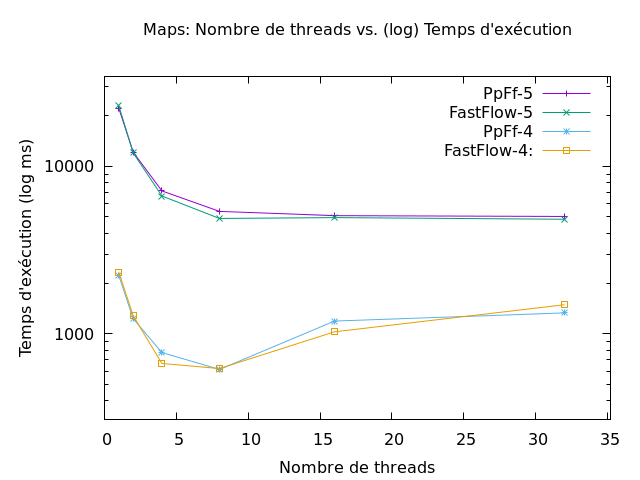
\includegraphics[width=1.0\textwidth]{Figures/graphe_temps_Java_Maps.png}
%      \caption{Les temps d'ex\'ecution pour \TT{MicroBenchmarkMaps} sur la machine \M1.}
%       \label{GrapheTempsMapsJava.fig}
%\end{figure}
%
%\begin{figure}
%\centering
%     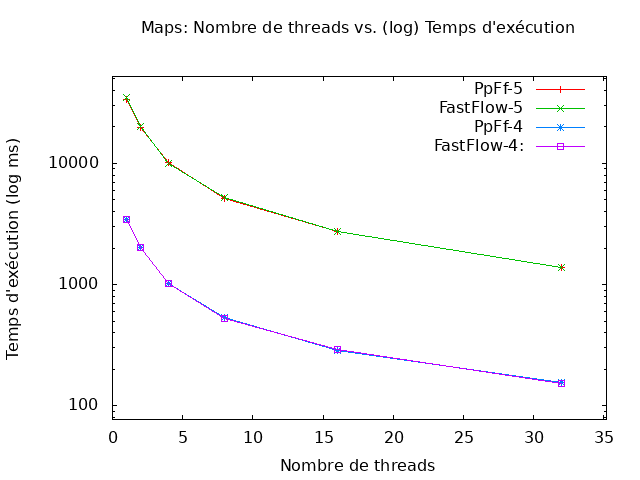
\includegraphics[width=1.0\textwidth]{Figures/graphe_temps_Japet_Maps.png}
%      \caption{Les temps d'ex\'ecution pour \TT{MicroBenchmarkMaps} sur la machine \M2.}
%       \label{GrapheTempsMapstJapet.fig}
%\end{figure}
%
%
%La figure~\ref{GrapheTempsMapsJava.fig} montre les r\'esultats des exp\'eriences sur la machine \M1\ alors que la figure~\ref{GrapheTempsMapstJapet.fig} montre les r\'esultats des exp\'eriences sur la machine \M2. On constate un faible surco\^ut
%introduit par \TT{PpFf} sur la machine \M1. Ce surco\^ut est plus \'evident lorsque la surcharge du calcul est moins grande. Pourtant, les surco\^uts introduits par \TT{PpFf} par rapport \`a \TT{FastFlow} restent faibles --- c'est ce qui explique, surtout dans la figure~\ref{GrapheTempsMapstJapet.fig}, que les lignes du graphe pour \TT{PfFf} et \TT{FastFlow}, tant avec 4 que 5 \emph{threads}, soient quasiment identiques~: la plus grande diff\'erence entre les temps d'ex\'ecutions de deux applications est de 300~ms. Le volume de traitement des deux applications est tr\`es grand. Le pipeline traite 100~000 \'el\'ements et l'algorithme de calcul appliqu\'e \`a chaque \'el\'ement consiste \`a incr\'ementer une valeur de 0 \`a 10~000 dans le cas avec la granularit\'e 4, ou de 0 \`a 100~000 avec la granularit\'e 5. Or, en prenant en consid\'eration ce grand volume de traitement des deux applications, ces 300~ms semblent n\'egligeables.


\section{Discussion des résultats et limites de \ppff}



\begin{figure}
\grapheH{WordCount-temps-java-2001-40-1345}

\grapheH{WordCount-temps-c34581-2003-40-1345}

\caption[Les temps d'exécution des programmes pour \TT{WordCount}
<<optimisé>> sur les machines \M1 et \M2.]{Les temps d'exécution des
programmes pour \TT{WordCount} <<optimisé>> sur les machines \M1 et
\M2. L'axe des $x$ indique le nombre de mots traités. L'axe des $y$
indique le temps d'exécution, en millisecondes.}
\label{WordCount-merged-temps.fig}
\end{figure}

\begin{figure}
\grapheH{WordCount-debits-java-2001-40-1345}

\grapheH{WordCount-debits-c34581-2003-40-1345}

\caption[Les debits des programmes pour \TT{WordCount}
<<optimisé>> sur les machines \M1 et \M2.]{Les debits des
programmes pour \TT{WordCount} <<optimisé>> sur les machines \M1 et
\M2. L'axe des $x$ indique le nombre de mots traités. L'axe des $y$
indique le debits, en millirs de mots traités par second.}
\label{WordCount-merged-debit.fig}
\end{figure}
